%----------------------------------------------------------------------

% Template for TECHNICAL REPORTS at Inst. for Computer Graphics

% and Vision (ICG), Graz University of Technology, Austria:

% style file 'techrep_icg.sty'

%

% author:  Pierre Elbischger

% email:   pierre.elibschger@icg.tu-graz.ac.at

% created: 13.11.2003

% last revision: 25.11.2003

%----------------------------------------------------------------------

% The template contains a number of LaTeX commands of the form :

%

% \command{xyz}

%

% In order to complete this abstract, fill in the blank fields between

% the curly braces or replace already filled in fields with the

% requested information.

%

% e.g. in order to add an abstract title, replace

% \title{}    with   \title{Evidence of Solitons in Tedium Diboride}

%

% The \author and \address commands can take an optional label

% in square brackets of the form :

%

% \command[label]{}

%

% The text of the abstract should be inserted between the two commands

% \begin{abstract} and \end{abstract}.

%

% Please leave all commands in place even if you don't fill them in.

%

%----------------------------------------------------------------------

% Do not alter the following two lines

\documentclass[12pt,a4paper]{article}               % I'm using a double-sided book style

      

\usepackage{techrep_icg}
\usepackage{array}
\usepackage{booktabs}
\usepackage{lscape}


% package 'graphicx' is automatically included depending on the

%   used compiler (latex, pdflatex), don't include it!!!



\begin{document}

%----------------------------------------------------------------------



%\reportnr{xxx}               % Number of the technical report

\title{Final Report} % Title of technical report

\subtitle{Camera relocalization using regression random forest} % Subtitle of technical report (use small letters only)

\repcity{Graz}            % City where the report was created

\reportnr{1}

\repdate{\today}          % Date of creation

\keywords{Report, Technical report, template, ICG} % keywords that appear below the abstract



%----------------------------------------------------------------------

% List of authors

%

% List each author using a separate \author{} command

% If there is more than one author address, add a label to each author

% of the form \author[label]{name}.  This label should be identical to

% the corresponding label provided with the \address command

% N.B. It is not possible to link an author to more than one address.

%

\author[ICG]{Thomas Pietsch 0930557}
\author[ICG]{Bernhard Rapp 0830250}


%----------------------------------------------------------------------

% List of addresses

%

% If there is more than one address, list each using a separate

% \address command using a label to link it to the respective author

% as described above


\newcommand{\TUGn}{Graz University of Technology}

\address[ICG]{Inst. for Computer Graphics and Vision \\ \TUGn, Austria}



%----------------------------------------------------------------------

% Information about the contact author

% if \contact is not defined (uncommented) or empty, the contact

%  information on the title page is suppressed.



% Name of contact

\contact{Thomas Pietsch}

% Email address of contact - do not use any LaTeX formatting here

\contactemail{thomas.pietsch@student.tugraz.at}



%----------------------------------------------------------------------

% Do not alter the following line



\section{Project Proposal}

\subsection{Introduction} % (fold)
\label{sub:intro}
First, a regression forest based on the Piotr Dollar toolbox \cite{piotr} will be implemented. The Matlab code for the Piotr Dollar toolbox is readily available and we will adapt the random classification forest to create a regression forest. Therefore the split function and output has to be modified.

Secondly the implementation itself should be evaluated, to make a statement to the general performance of the implementation.

After that the implementation should be adapted for camera relocalization as shown by Shotton et al \cite{shotton}. The adapted implementation is further evaluated using the dataset given by Shotton et al.

\subsubsection{Regression Random Forest}
\label{rrf_intro}
The weak learner given by equation (\ref{eqn:weaklearner}) also called split function splits the data into a left and right dataset, by thresholding.

\begin{eqnarray}\label{eqn:weaklearner}
  h(\mathbf{p};\mathbf{\theta}_n) = [ f_{\phi_n}(\mathbf{p}) \geq \tau_n ]
\end{eqnarray}

Such a threshold can be optimized by minimization of the objective function

\begin{eqnarray} \label{eqn:objectiv_function}
  Q(S_n,\theta) = V(S_n) - \sum_{d\in\{L,R\}}{\frac{|S_n^d(\theta)|}{|S_n|}V(S_n^d(\theta))}
\end{eqnarray}

\begin{eqnarray}
  V(S) = \frac{1}{|S|} \sum_{(\mathbf{p},\mathbf{m}) \in S}{||\mathbf{m} - \mathbf{\bar m}||_2^2}
\end{eqnarray}

By computing the mean and variance at each leaf, the probability of the output value is given as well as the output value itself is given simply by the mean value.
Because several trees are included in a forest the output of all trees have to be averaged.

\subsection{Implementation} % (fold)
\label{sub:implementation}
To achieve the defined goal, the Piotr Dollar toolbox \cite{piotr} was adopted. To be more precise the Objective function as given in equation (\ref{eqn:objectiv_function}) was added. Also variance and mean were added as component of the forest structure, while the mean value can be interpreted as the regression result of each tree.

\subsubsection*{Regression Forest} % (fold)
\label{ssub:regression_forest}

% subsubsection regression_forest (end)

\subsubsection{Evaluation} % (fold)
\label{ssub:camera_relocalization}
First the implementation of a general Random Regression Forest was evaluated. To keep things simple, simple 2D functions were used to calculate an error as well as a visualization.
Some attributes were kept constant:
\begin{itemize}
	\item maxDepth = 50
  \item minChild = 1
\end{itemize}

For the general regression task, the number of input and the amount of trees per forest were varied. The implementation was tested with a one dimensional dataset: $cos(x*pi*4 + (x+1))^2$ which is shown in table ~\ref{tab:res_gen_cos}, and with a two dimensional dataset: $2*x + 3*y$ which is shown in table ~\ref{tab:res_gen_plane}

\begin{landscape}

\begin{table}[p]
\begin{tabular}{|c|c|c|c|}
\toprule
Datapoints & \multicolumn{3}{|c|}{trees} \\ \hline
\midrule
& 50 & 150 & 1500 \\ \hline
1000 & 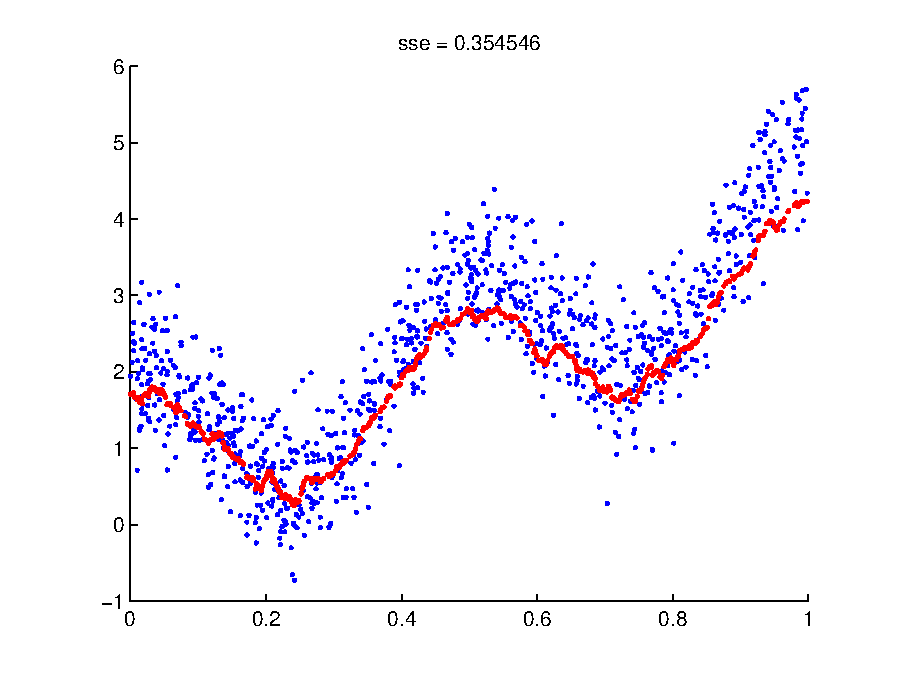
\includegraphics[width=0.5\textwidth, height=0.35\textheight]{fig/cos_1k_50} & 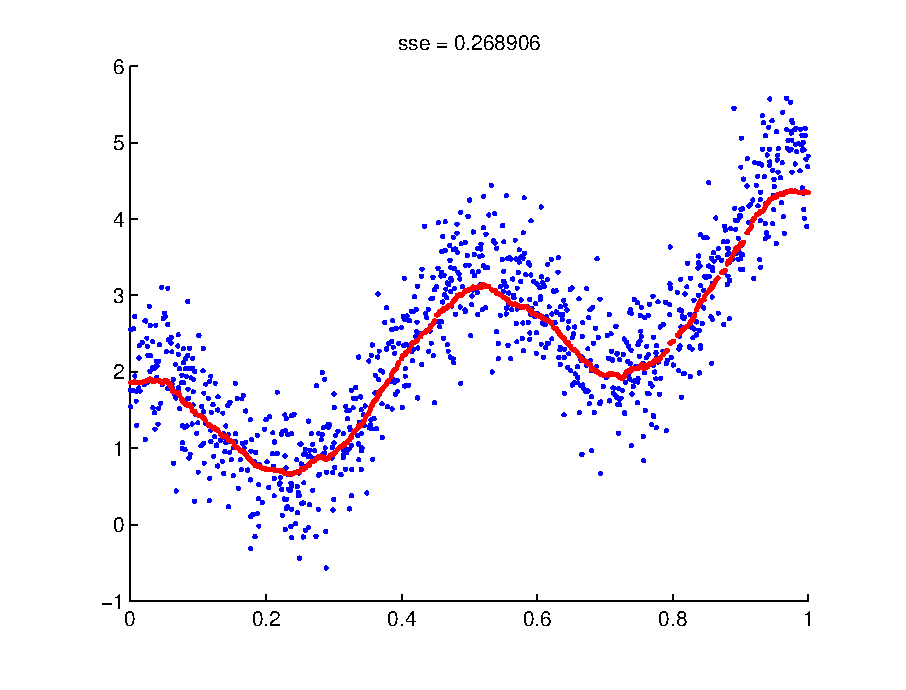
\includegraphics[width=0.5\textwidth, height=0.35\textheight]{fig/cos_1k_150} & 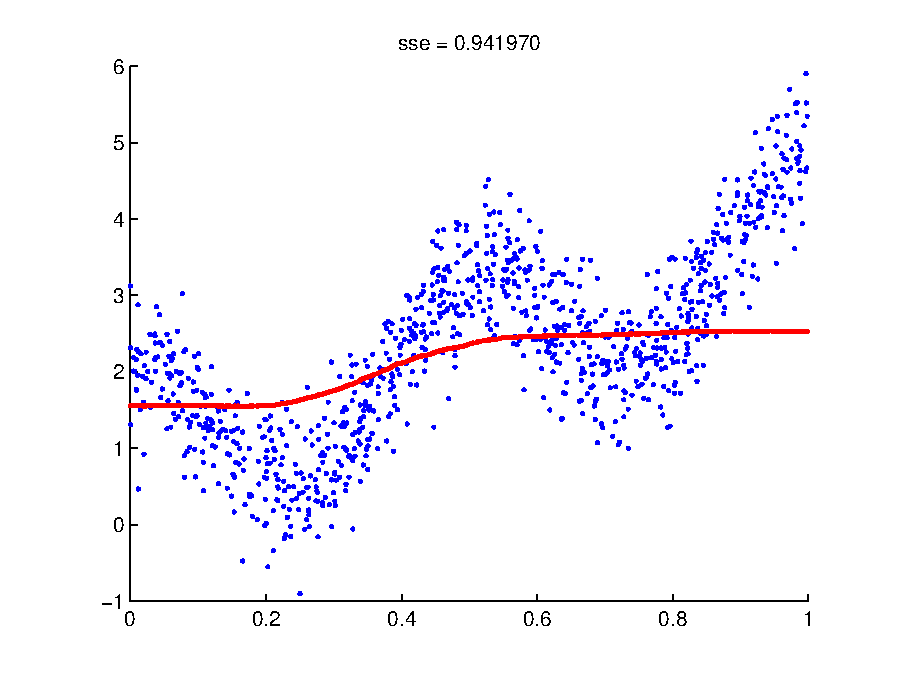
\includegraphics[width=0.5\textwidth, height=0.35\textheight]{fig/cos_1k_1500} \\ \hline
10000& 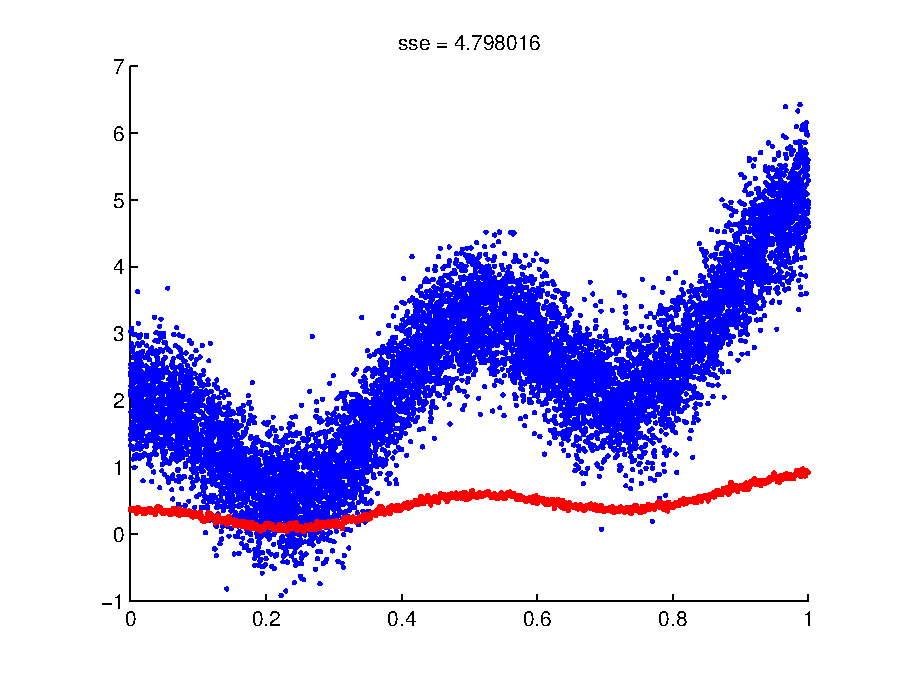
\includegraphics[width=0.5\textwidth, height=0.35\textheight]{fig/cos_10k_50} & 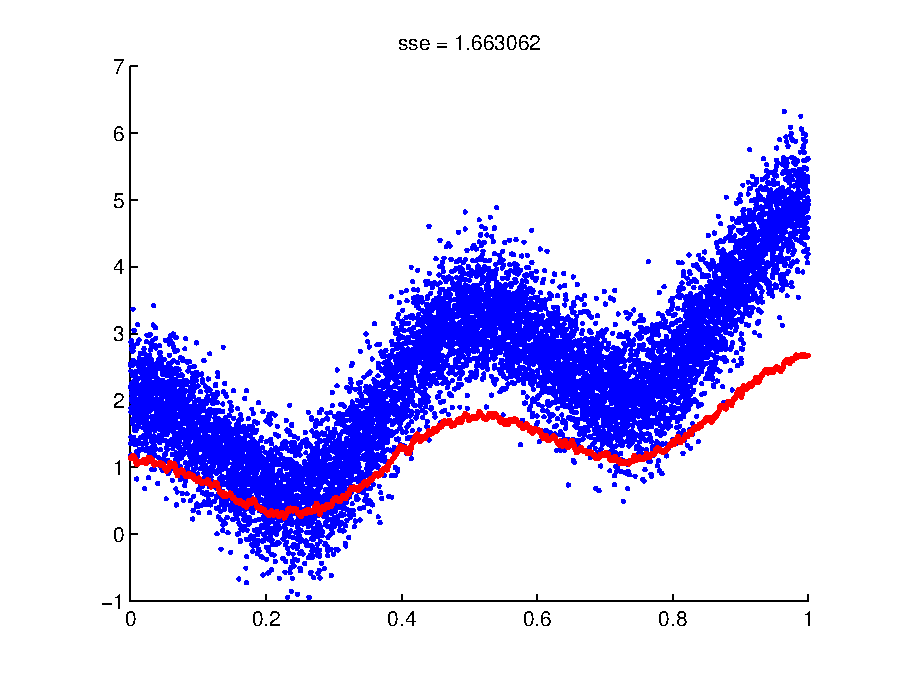
\includegraphics[width=0.5\textwidth, height=0.35\textheight]{fig/cos_10k_150} & 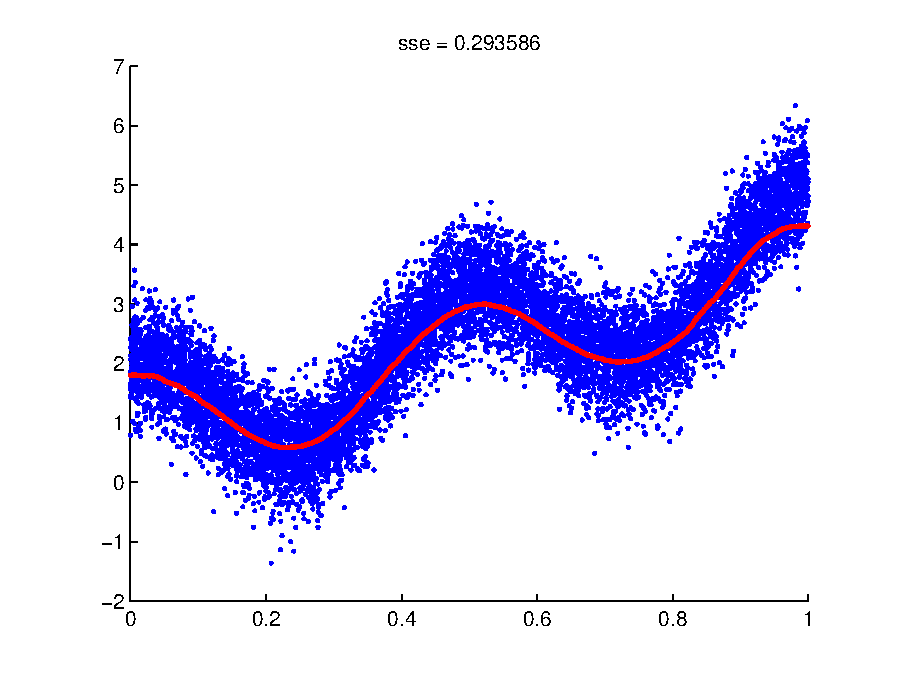
\includegraphics[width=0.5\textwidth, height=0.35\textheight]{fig/cos_10k_1500} \\ \hline
\bottomrule
\end{tabular}
\caption{The Table shows the results of varying the size of trees and size of input data. The images shows in red result of the forest, blue the labeled data. The used function was $cos(x*pi*4 + (x+1))^2$.}
\label{tab:res_gen_cos}
\end{table}

\begin{table}[p]
\begin{tabular}{|c|c|c|c|}
\toprule
Datapoints & \multicolumn{3}{|c|}{trees} \\ \hline
\midrule
& 50 & 150 & 1500 \\ \hline
1000 & 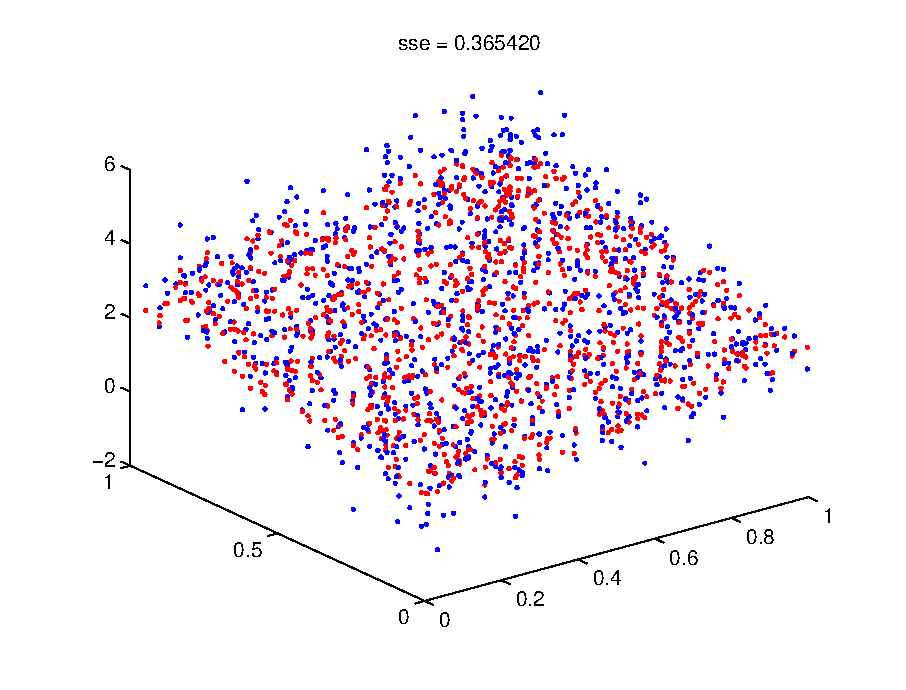
\includegraphics[width=0.5\textwidth, height=0.35\textheight]{fig/plane_1k_50} & 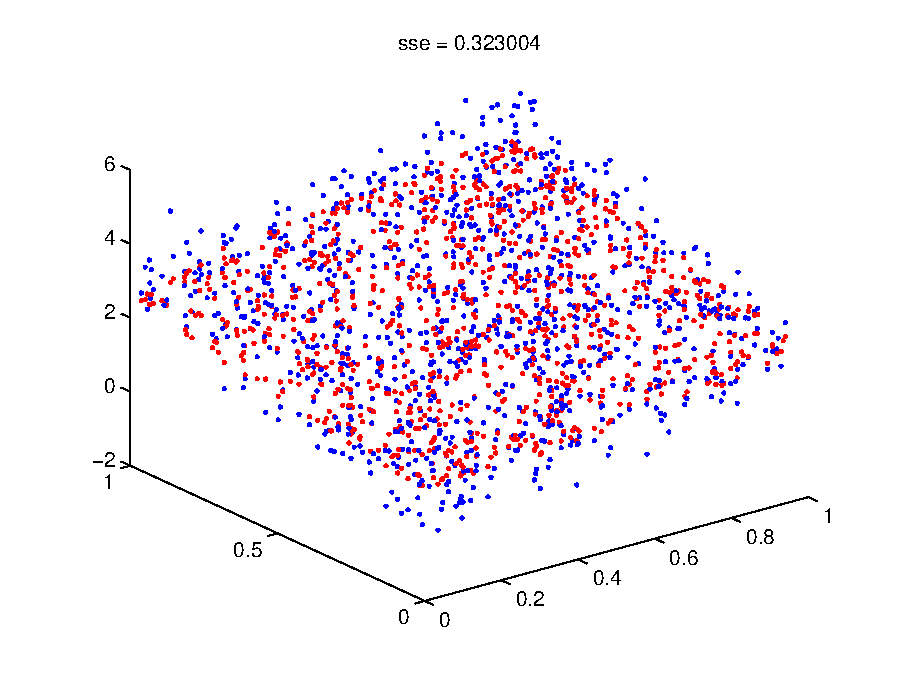
\includegraphics[width=0.5\textwidth, height=0.35\textheight]{fig/plane_1k_150} & 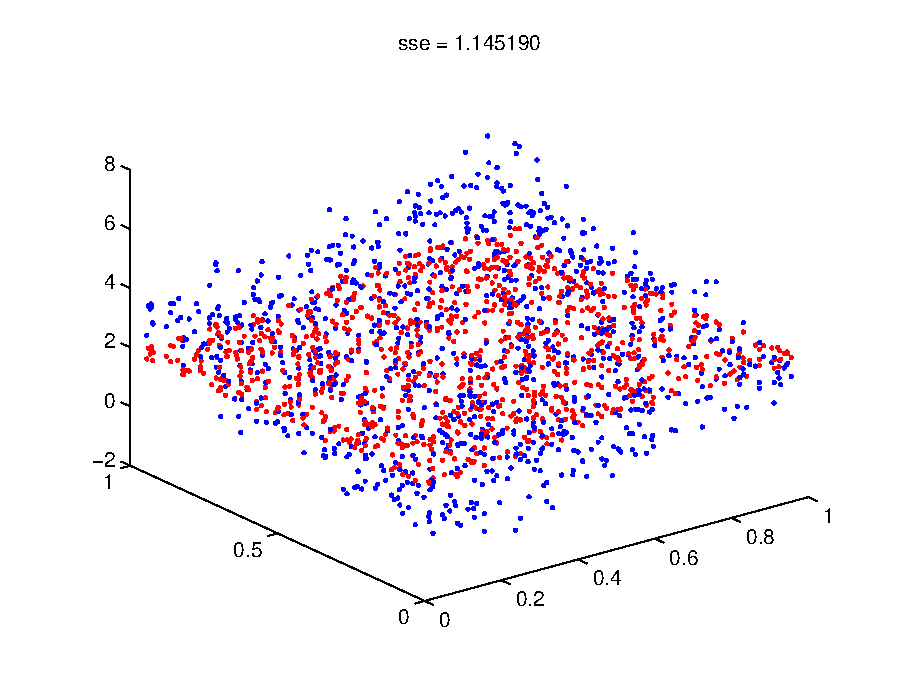
\includegraphics[width=0.5\textwidth, height=0.4\textheight]{fig/plane_1k_1500} \\ \hline
10000& 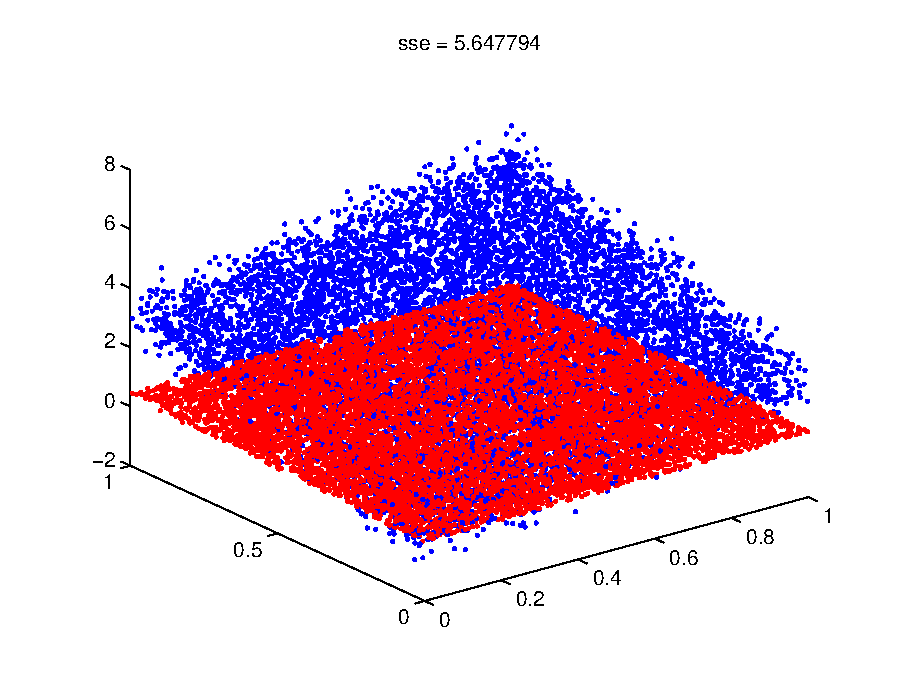
\includegraphics[width=0.5\textwidth, height=0.35\textheight]{fig/plane_10k_50} & 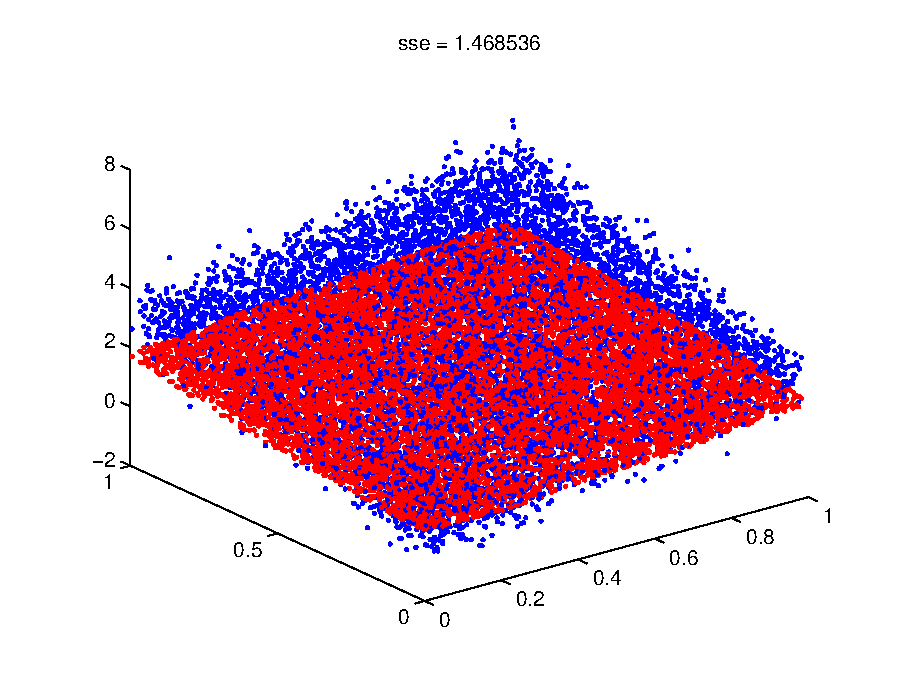
\includegraphics[width=0.5\textwidth, height=0.35\textheight]{fig/plane_10k_150} & 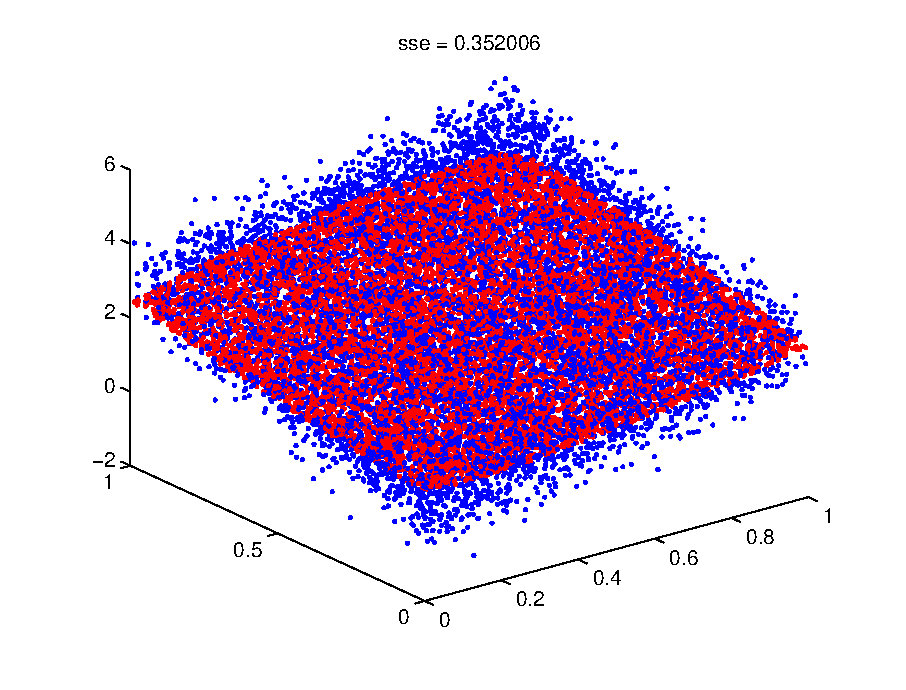
\includegraphics[width=0.5\textwidth, height=0.35\textheight]{fig/plane_10k_1500} \\ \hline
\bottomrule
\end{tabular}
\caption{The Table shows the results of varying the size of trees and size of input data. The images shows in red result of the forest, blue the labeled data. The used function was a plane: $2*x + 3*y$}
\label{tab:res_gen_plane}
\end{table}

\end{landscape}

\subsubsection*{Camera relocalization} % (fold)
\label{ssub:relocalization}
After the general random regression forest, the implementation was extended to perform an camera relocalization task, as shown by Shotton et al. \cite{shotton}. Here the results are presented in table ~\ref{tab:res_reallocation} in order the coordinates in real world coordinates.

\begin{table}[p]
\begin{tabular}{|c|c|c|c|c|c|c|c|}
\toprule
\hline Tree Configuration & \multicolumn{3}{|c|}{Ground truth} & \multicolumn{3}{|c|}{Prediction} & RSS \\ \hline
& x & y & z & x & y & z & \\ \hline
\midrule
\hline
150 & -466.7 & 530.4 & 1446.7 & 305.0 & 370.1 & 450.1 & 4.8289e+11  \\ \hline
150 & -483.8 & 509.9 & 1397.5 & 281.6 & 384.3 & 500.3 & 5.4586e+11  \\ \hline
150 & -145.3 & 709.7 & 843.3 & 301.8 & 407.6 & 499.6 & 2.6319e+11  \\ \hline
150 & 429.4 & 472.3 & 49.0 & 297.0 & 394.9 & 498.4 & 5.1679e+10  \\ \hline
50 & -6.4 & 424.0 & 1401.8 & 242.6 & 371.2 & 517.4 & 5.5096e+11  \\ \hline
50 & -48.2 & 503.6 & 1241.9 & 362.0 &  220.7 & 501.4 & 4.2114e+11 \\ \hline
50 & -107.1 & 634.0 & 1054.0 & 308.4 & 408.9 & 503.8 & 3.5035e+11 \\ \hline
50 & 360.2 & 28.7 & 137.9 &  274.8 & 384.9 & 537.4 & 1.5420e+10 \\ \hline
\bottomrule
\end{tabular}
\caption{The Table shows 5 randomly chosen results of two different trees. Here the data size is fixed to the image size 640x480. RRS being the residual sum of squares. Note that the coordinates are given in real world coordinates.}
\label{tab:res_reallocation}
\end{table}

\subsection{Problems}

Because the relocalization forest should dice at each node the parameters new, it was not possible to calculate the input data in advance. Therefore the decision was made to use a matrix of function handles to perform the calculation of the input data in each node. This has to be done at the training and by applying the forest to actual calculate the result. Because of this the implemenation is much slower than the original classification regression forest. To improve performance at the apply state, it might be possible to calculate the input data only for those pixels which are actual used instead of every pixel. Because in a leaf or deeper nodes, 307200 data points or pixels are calculated but maybe only 4 are used!

Additionally only one image (color as well as its corresponding depth) is used for training and applying instead of the whole image base. This leads also to the bad performance in terms of a big error. 


% ============================================================
% Bibliography
% ============================================================
\clearpage
\renewcommand{\leftmark}{}



\bibliographystyle{plain}
%\addcontentsline{toc}{chapter}{Bibliography}
%\bibliographystyle{plain}
\bibliography{./bibtex}

\end{document}

%----------------------------------------------------------------------

